\chapter{Dataset Generation and Parameters}
\label{ch:dataset_generation}
This chapter presents the choice of parameters for the datasets used in the context of this thesis.

\section{Primary Dataset}
The parameters which were used to generate the primarily used dataset for training, validation, and various evaluations
on the test set are listed in \autoref{tab:dataset_parameters}.

\begin{table}
    \centering
    \caption{Dataset Generation Parameters for \( \DMain \)}
    % \footnotesize
    \begin{tabularx}{\textwidth}{@{}lX@{}}
    \toprule
    \textbf{Parameter} & \textbf{Details} \\
    \midrule
    Dataset Size  \( \|\mathcal{D}\| \) & \( \num{2e6} \) samples \\
    Train-Validation-Test Ratios &
    \begin{tabular}{@{}lll@{}}
    0.6 (Training) & 0.2 (Validation)  0.2 (Test) \\
    \( \|\DTrain\| = \num{1.2e6}\) & \( \|\DVal\| = \|\DTest\| = \num{4e5}\)
    \end{tabular} \\
    \addlinespace
    \midrule
    \textbf{Signal Characteristics} & \\
    Signal Distribution &
    \begin{tabular}{@{}ll@{}}
    \( N \) & Relative Share \\
    \midrule
    0 & \( 1/6 \) \\
    1 & \( 1/6 \) \\
    2 & \( 1/6 \) \\
    3 & \( 1/6 \) \\
    4 & \( 1/6 \) \\
    5 & \( 1/6 \)
    \end{tabular} \\
    SNR Distribution & Random Uniform \\
    Frequency Bounds & \( f_{\text{c}} \): 1.15 \si{\giga\hertz} (Fixed frequency for all signals) \\
    SNR Bounds & \( [2.5, 30) \) dB \\
    SIR Bounds & \( [0, 29) \) dB \\
    Azimuth Range & \( [0^\circ, 360^\circ) \) \\
    Elevation Range & \( [0^\circ, 90^\circ) \) \\
    Minimum Azimuth Difference  & \( 5^\circ \) \\
    \addlinespace
    \midrule
    \textbf{Antenna Array Configuration} & \\
    Array Type & \glsdesc{uca} \\
    \# Elements \( M \) & 9 \\
    Center Element & False \\
    Diameter \( d_{\text{ant}} \) & 0.26 m \\
    Parameters \( a, b \) & \( a = 1 \), \( b = 0 \) \\
    \addlinespace
    \midrule
    \textbf{Subarray Sampling} & \\
    Status & Enabled \\
    \# RF Paths \( L \) & 3 \\
    Mode & Covariance Matrix \\
    \addlinespace
    \midrule
    \textbf{Preprocessing and Measurement} & \\
    \# Snapshots \( K \) & 100 \\
    Sampling Rate \( f_{\text{s}} \) & 12.8 \si{\kilo\hertz}  \\
    Bandwidth \( f_{\text{B}} \) & 1 \si{\kilo\hertz} \\
    Noise Level \( L_{\eta} \) & -120 \( \si{\decibel}_{(\si{\micro\volt})} \) \\
    Preprocess Measurement Vector & Differencing: True \\
    \bottomrule
    \end{tabularx}
    \label{tab:dataset_parameters}
\end{table}

\subsection{Choice of Parameters}
The dataset \( \DMain \) employs \textit{sub}array sampling with \( L = 3 \) RF paths, and performs the accumulation of the \( K = 100 \) snapshots by
averaging the single sub-array covariance matrices according to~\autoref{subsec:ImpactOnTheCovarianceMatrix}. \\
It consists of \( \num{2e6} \) samples, and was generated adhering to the data model described in \autoref{chap:DataModel}.\\
The individual dataset split sizes for training, validation, and testing are chosen to follow the common practice of a 60:20:20 split.

The model order \( N \) is uniformly distributed with a relative share of \( 1/6 \) for each \( N \in \NSet = \{0, \ldots, 5\} \).
A predecessor to \( \DMain \), employed an approximately Gaussian distribution with respect to the model order.
However, datasets with class imbalances should be avoided, unless the imbalances are a characteristic of the problem and
known a priori. The evaluation on this dataset would also have provided an unfair advantage to the neural networks over
the traditional methods, as the latter are incapable of considering various statistical distributions from previously
observed data into the decision-making process.

Only a single carrier frequency \( f_{\text{c}} = 1.15 \si{\giga\hertz} \) is used, to reduce the complexity of the parameter space for
ease of interpretation. \\
The diameter of the \gls{uca} \( d_{\text{ant}} \) are chosen such that the antenna aperture
becomes \( D \approx 1 \), given that \( D = f_C \cdot d_{\text{ant}} / c_0\).\\
The antenna parameters \( a \) and \( b \) are set such that the antenna elements exhibit isotropic radiation patterns,
simplifying the directivity to a constant \( c(\bfT, f_C) = const. = 1 \).

The noise level \( L_{\eta} \) is set to -120 \( \si{\decibel}_{(\si{\micro\volt})} \), which corresponds to a noise variance
of \( \sigma^2_{\eta} = 1 \si{\micro\volt\squared} \).

\newpage{}
\subsubsection{SNR and SIR Distributions}
\label{subsub:snr_sir_distrib}

The statistical distributions of the \glspl{snr} and \glspl{sir} hold pivotal roles in many fields of signal processing.
Its significance in the context of model order estimation in \gls{ddf} systems cannot be overstated, as will be detailed
in the following chapters. \\
Another parameter with even greater influence on the performance of model order estimation methods is the model order \( N \).

Understanding the interplay between SNR/SIR distributions and the model order is hence imperative for a
meaningful and comprehensive performance evaluation of various \gls{moe} methods against the backdrop of varying
SNR/SIR conditions, particularly as explored in \autoref{evaluation_results}.\\
For instance, the achieved test accuracy of a model order estimation method within a specific \( \SNRmin \) range, \( \SNRmin + \Delta\SNR \),
might appear phenomenal. However, further analysis of the sample density with in this range might reveal that the achieved
accuracy does not hold any significance due to the low density within this range. \\
Furthermore, an inconsiderate conclusion about the causal relationship between the maximum SNR, \( \SNRmax \), and the occurence of
some extraordinary important markers might be drawn, that later turns out to be only a correlation, whose actual cause
is the model order \( N \).\\

The \glspl{snr} of each signal are drawn from a random uniform distribution \( \mathcal{U}(l, u) \),
which is characterized by its lower \gls{snr} and upper bounds, which are defined in~\autoref{tab:dataset_parameters}.
The absolute amplitudes of the signals are subsequently calculated from the \gls{snr} levels, by adding them onto the
specified absolute%
\footnote{The utilized Python environment does currently not support varying noise floors. Considering the
relation between the noise floor and the behavior of the eigenvalues, this feature should be considered as a future extension.}
noise level \( L_\eta \), as per equations~\ref{eq:noise_amplitude} and~\ref{eq:signal_amplitude}.

\begin{align}
    \frac{\hat{a}_\eta}{1\si{\micro\volt}} &= 10^{\left(\frac{L_{\eta}}{20}\right)}
    \label{eq:noise_amplitude} \\
    \frac{\hat{a}_S}{1\si{\micro\volt}} &= \hat{a}_\eta \cdot 10^{\left(\frac{L_{\text{SNR}}}{20}\right)}
    \label{eq:signal_amplitude}
\end{align}

For ease of notation, we will henceforth refer to the \gls{snr} and \gls{sir} levels as per equations~\ref{eq:snr_min} to~\ref{eq:sir}.

\begin{align}
    \SNRmin &= 20 \lg \left(\frac{\hat{a}_{S, \min}}{\hat{a}_\eta}\right) = 10 \lg \left(\frac{\sigma_{S, \min}^2}{\sigma_{\eta}^2}\right) \label{eq:snr_min}\\
    \SNRmax &= 20 \lg \left(\frac{\hat{a}_{S, \max}}{\hat{a}_\eta}\right) = 10 \lg \left(\frac{\sigma_{S, \max}^2}{\sigma_{\eta}^2}\right) \\
    \SIR &= 20 \lg \left(\frac{\hat{a}_{S, \max}}{\hat{a}_{S, \min}}\right) =    10 \lg \left(\frac{\sigma_{S, \max}^2}{\sigma_{S, \min}^2}\right) \label{eq:sir}
\end{align}

The dependence of the \( \SNRmin \), \( \SNRmax \) and \( \SIR \) on the model order arises from the fact that
individual \( \SNR_i \) for \( i \in \{0, \ldots, N\} \) are independently sampled from \( \mathcal{U}(l,u) \).
Additionally, the definition of the \gls{sir} inherently necessitates the presence of more than one signal source to hold significance.\\
Although it's challenging to completely eliminate the profound influence of the model order on the subsequent analysis,
we aim to offer a brief discussion on how the model order \( N \) shapes the density estimates of \( \SNRmin \), \( \SNRmax \),
and \( \SIR \). \\
The following considerations lay the foundation for a meaningful understanding of the performance evaluation of
the \gls{moe} methods with respect to the \gls{snr} and \gls{sir}, which will be conducted in~\autoref{ch:evaluation_results},
and will also be of relevance in the context of addressing the initial challenges of eigenvalue-based \gls{moe} methods in~\autoref{sec:challenges_moe}.

All measures of interest are derived from the \( N \) dimensional vector of \gls{snr} values \( \bfm{\SNR} \in \mathbb{R}^N\):
\begin{align}
    \SNRmin & \sim \min\left(\SNR_0, \ldots, \SNR_N\right), \quad \SNR_n \sim  \mathcal{U}(l,u) & \text{for } N \geq 1 \\
    \SNRmax & \sim \max\left(\SNR_0, \ldots, \SNR_N\right) & \text{for } N \geq 1 \\
    \SIR & \sim \SNRmax - \SNRmin & \text{for } N \geq 2
    \label{eq:snr_sir_dist}
\end{align}


The foundational distribution for individual SNR values is the uniform distribution \(\SNR \sim \mathcal{U}(l,u)\),
characterized by the following \gls{pdf} and \gls{cdf}~\cite[Chapter 5.2]{blitzstein2019}:
\begin{align}
    f_{\mathcal{U}}(x)= \begin{cases} \frac{1}{u-l} & \text { if } l<x<u \\ 0 & \text { otherwise } \end{cases} \label{eq:uniform_pdf}\\
    F_{\mathcal{U}}(x)= \begin{cases} 0 & \text { if } x \leq l \\ \frac{x-l}{u-l} & \text { if } l<x<u \\ 1 & \text { if } x \geq u \end{cases}
    \label{eq:uniform_cdf}
\end{align}

By substituting the CDF of the uniform distribution \( F_{\mathcal{U}}(x) \) from~\autoref{eq:uniform_cdf} into the
order statistics equations for \( \SNRmin \) and \( \SNRmax \) (where \( F_{\SNRmin} = F_{(1)} \) and \( F_{\SNRmax} = F_{(N)} \)),
we obtain the CDFs of \( \SNRmin \) and \( \SNRmax \) for \( N > 1 \).
This process is detailed in~\cite[Chapter 8.6]{blitzstein2019}:

\begin{equation}
    F_{\SNRmin}(x) = 1 - \left(1 - \frac{x-l}{u-l}\right)^N \quad \text{for } x \in [l, u]
\end{equation}

\begin{equation}
    F_{\SNRmax}(x) = \left(\frac{x-l}{u-l}\right)^N \quad \text{for } x \in [l, u]
\end{equation}

The PDFs of \( \SNRmin \) and \( \SNRmax \) for \( N > 1 \) are subsequently obtained by differentiating the CDFs with respect to \( x \):
\begin{equation}
    f_{\SNRmin}(x) = \frac{d}{dx}F_{\SNRmin}(x) = \frac{N}{u - l} \left(1 - \frac{x - l}{u - l}\right)^{N-1} \quad \text{for } x \in [l, u]
    \label{eq:snrmin_pdf_nge1}
\end{equation}

\begin{equation}
    f_{\SNRmax}(x) = \frac{d}{dx}F_{\SNRmax}(x) = \frac{N}{u - l} \left(\frac{x - l}{u - l}\right)^{N-1} \quad \text{for } x \in [l, u]
    \label{eq:snrmax_pdf_nge1}
\end{equation}

To validate the soundness of the obtained PDFs, the theoretical PDFs of \( \SNRmin \) and \( \SNRmax \) were compared to
the density estimates of \( \SNRmin \) and \( \SNRmax \) obtained from the \( \DMain_{(\text{test})} \) dataset.
\begin{figure}[H]
    \centering
    \subfloat[\( f_{\SNRmin} \)]{{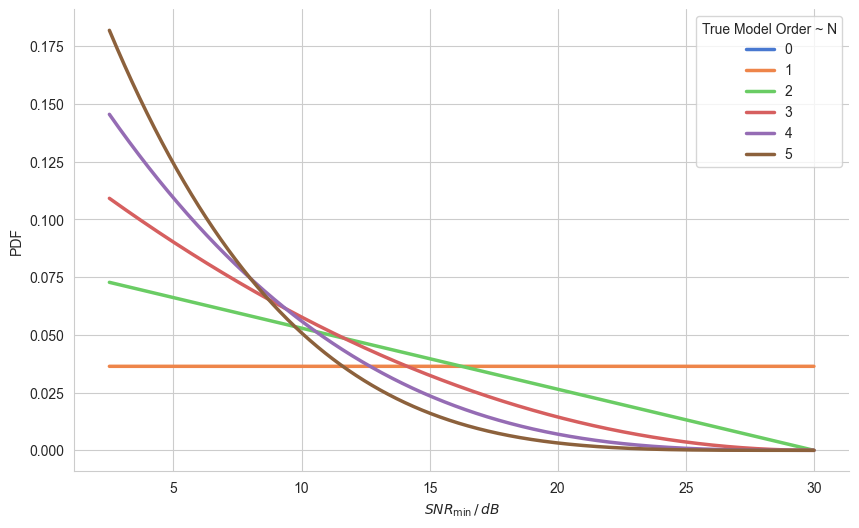
\includegraphics[width=0.5\textwidth]{figures/07_Evaluation/snr_hist/pdf_snr_min.png}}}
    \subfloat[\( \hat{f}_{\SNRmin} \)]{{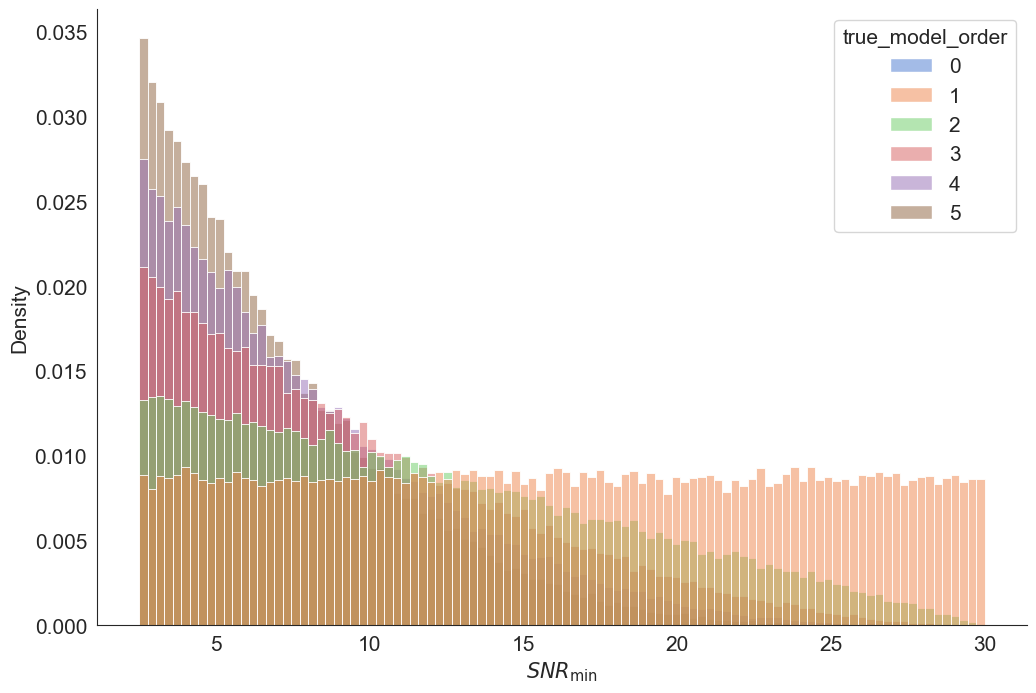
\includegraphics[width=0.5\textwidth]{figures/07_Evaluation/snr_hist/min_N.png}}}
    \newline
    \subfloat[\( f_{\SNRmax} \)]{{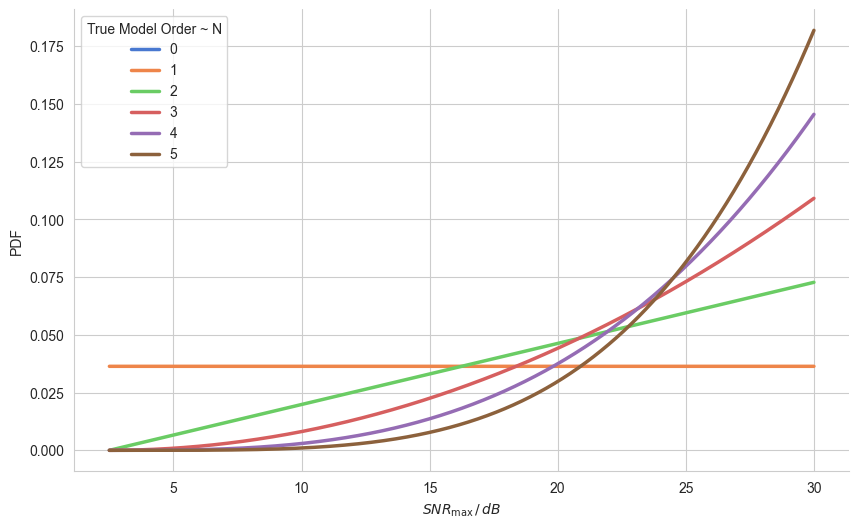
\includegraphics[width=0.5\textwidth]{figures/07_Evaluation/snr_hist/pdf_snr_max.png}}}
    \subfloat[\( \hat{f}_{\SNRmax} \)]{{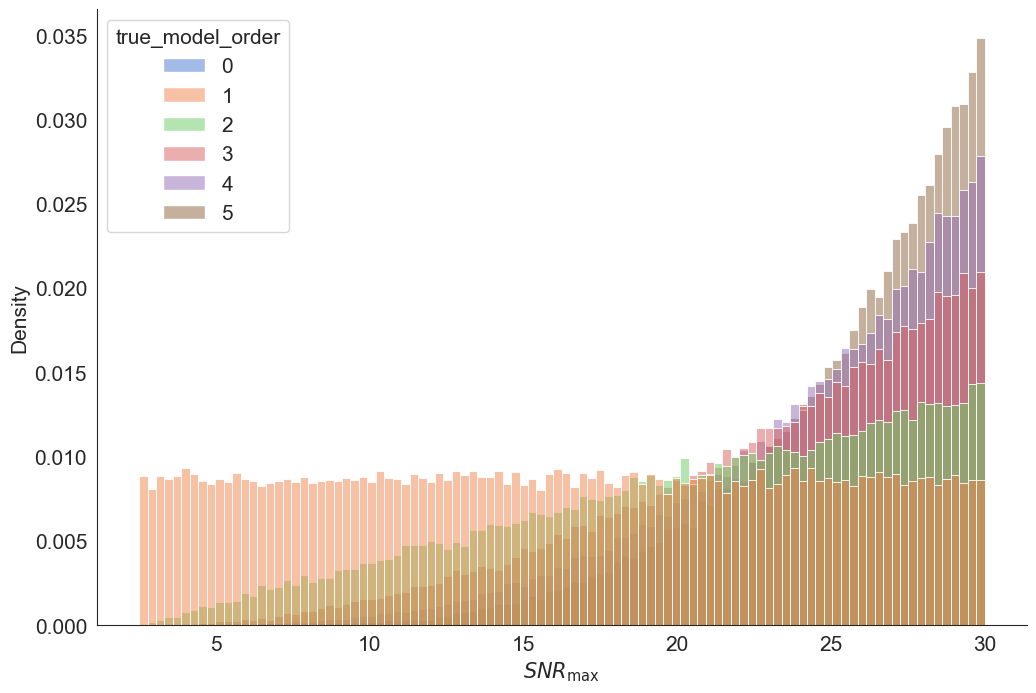
\includegraphics[width=0.5\textwidth]{figures/07_Evaluation/snr_hist/max_N.png}}}
    \caption{Theoretical \glspl{pdf} (a, c) and empirical density estimates (b, d) for \( \SNRmin \) and  \( \SNRmax \).}
    \label{fig:snr_pdf}
\end{figure}

To obtain the PDF of the \( \SIR \) distribution for \( N \geq 2 \), a convolution of the PDFs of the random variables \( \SNRmin \) and \( \SNRmax \)
is required. The convolution of the two PDFs is given by:
\begin{equation}
    f_{\SIR}(z) = \int_{-\infty}^{+\infty} f_{\SNRmax}(x) f_{\SNRmin}(z - x) \, dx
    \label{eq:sir_pdf}
\end{equation}

Numerical integration of the convolution in~\autoref{eq:sir_pdf} yielded the following PDF for \( \SIR \)~\cite[Chapter 8.2]{blitzstein2019}:
\begin{figure}[H]
    \centering
    \subfloat[\( f_{\SIR} \)]{{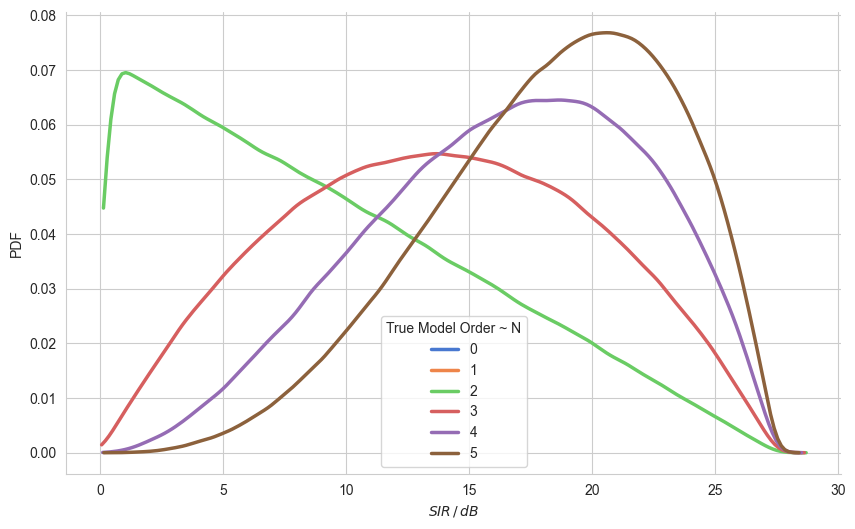
\includegraphics[width=0.5\textwidth]{figures/07_Evaluation/snr_hist/pdf_sir.png}}}
    \subfloat[\( \hat{f}_{\SIR} \)]{{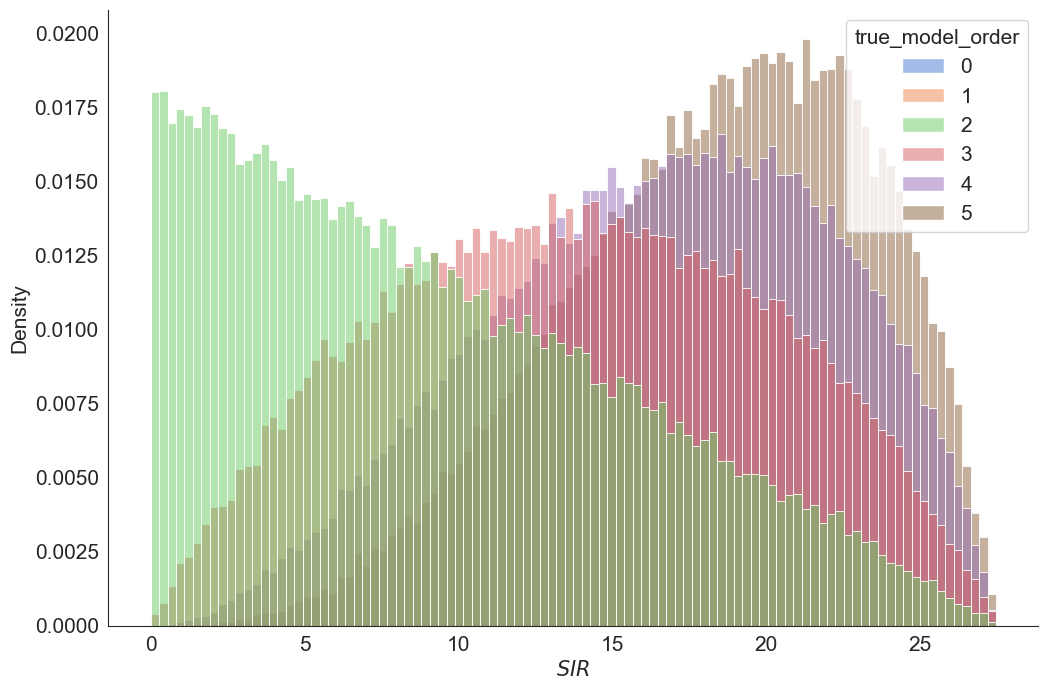
\includegraphics[width=0.5\textwidth]{figures/07_Evaluation/snr_hist/sir_N.png}}}
    \caption{Theoretical \glspl{pdf} (a) and empirical density estimates (b) for \( \SIR \).}
    \label{fig:sir_pdf}
\end{figure}
%%%%%%%%%%%%%%%%%%%%%%%%%%%%%%%%%%%%%%%%%%%%%%%%%%%%%%%%%%%%%%%%%%%%%%%%%%%%%%%%%%%%%%%%%%%%%%%%%%%%%%%%%%%%%%%%%%%%%%%%

\section{Supplementary Dataset Variations}
\label{sec:supplementary_datasets}
To further our understanding, we generated additional datasets with parameters largely mirroring those in \autoref{tab:dataset_parameters}.
These datasets, however, vary in the number of snapshots \( K \) or employ a fully sampled covariance matrix, as delineated below:

\begin{align*}
    \DKvar &\leftrightarrow  K = var. \land K \in [1, 1000]\\
    \DCoh &\leftrightarrow  \text{uses fully sampled covariance matrix}\\
\end{align*}


The sampling strategy for \( K \) within \( \mathcal{D}^{\{K_{var.},\text{Sub}\}} \) is as follows:

\[
    K_{var} =
\begin{cases}
    \text{2000 samples, increment of 1,} & \text{for } 1 < K \leq 10, \\
    \text{20000 samples, increment of 5,} & \text{for } 10 < K \leq 100, \\
    \text{20000 samples, increment of 10,} & \text{for } 100 < K \leq 200, \\
    \text{20000 samples, increment of 25,} & \text{for } 200 < K \leq 1000.
\end{cases}
\]

Post-generation, the dataset underwent uniform resampling with a step size of 25 to ensure a balanced distribution across
the spectrum of snapshots, thus providing a robust basis for model evaluation.


